\section{Chaîne}
\q{Tracer la courbe $y = f(x, t)$ pour une vitesse $c = 2$ et des temps espacés
  de $t = 0.2*k$ avec $t \leq 5$.}

\codeFromFileT{main.py}{section-03/qa.py}

En exécutant :
\codeFromFile{section-03/qb.py}
J'obtiens :
\begin{center}
  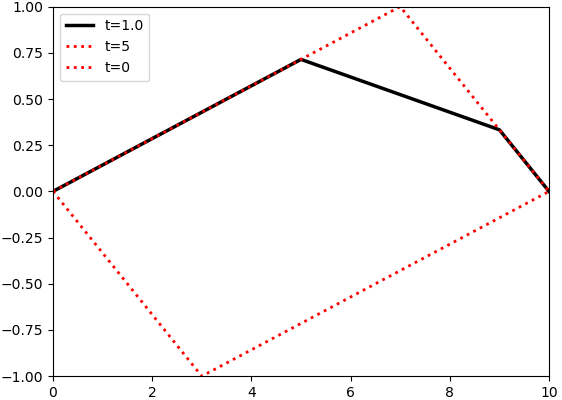
\includegraphics[scale=0.5]{section-03/qc-1.png}
  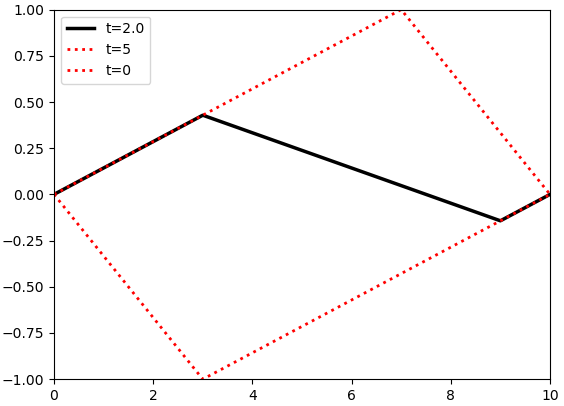
\includegraphics[scale=0.5]{section-03/qc-2.png}
  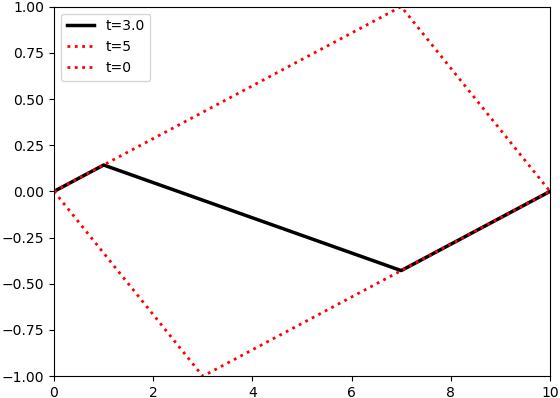
\includegraphics[scale=0.5]{section-03/qc-3.png}
  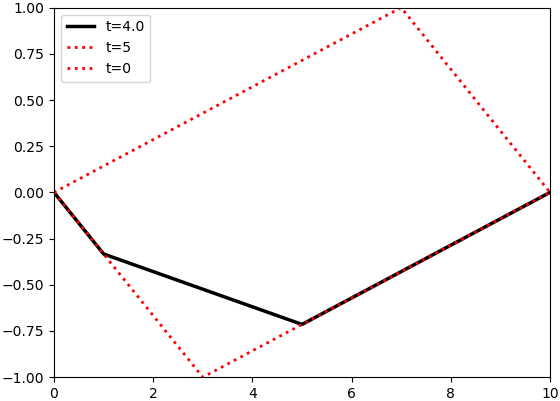
\includegraphics[scale=0.5]{section-03/qc-4.png}
\end{center}
